\documentclass[a4]{article}
\usepackage{tikz}
\usepackage{pgf}
\usepackage{singlelinetikz}
\usepackage{setspace}
\usepackage[most]{tcolorbox}
\usepackage{makeidx}
\usepackage{array}
\usepackage{booktabs}
\usepackage{amsmath}
\usepackage{amssymb}
\usepackage{float}
\usepackage[a4paper, left=3cm, right=3cm, top=2cm]{geometry}
\usepackage{xspace}
\usepackage{graphicx}
\usetikzlibrary{angles}
\usepackage{xcolor}
\usepackage{fancyvrb}
\definecolor{myblue}{RGB}{72,61,139}
\definecolor{mygray}{RGB}{140,140,140}
\tcbset{colback=yellow!10!white,arc=0.2mm,width=\linewidth,
before={\par\pagebreak[0]\medskip\parindent=0pt},after=\hfill, fonttitle=\bfseries ,colframe=yellow}
\newtcolorbox{examplebox}[1][]{
 %colframe=black!10!white,
  boxrule=0pt,frame hidden,
top=0mm, bottom=0mm,
%after=% <----- remove the default \par
}
\newcommand*\Tikz{\textup{Ti\textit kZ}\xspace}
\title{\texttt{singleline} \\ Single-line diagrams with TikZ\\
v. 1.0.0\vspace{1cm}}
\author{Author: \vspace{1cm}Isabelle Brandherm}
\date{\today}
\makeindex
\begin{document}
\maketitle
\tableofcontents
\pagebreak
\section{Introduction}
The \texttt{singleline} package is a \Tikz based \LaTeXe  \ package for drawing single-line diagrams of three-phase power systems. It consists of a collection of drawing commands and nodes of the most used circuit symbols. The package is based on the EN 60617-2/-11 standard.
  
To use \verb+singleline+-commands enclosure in a \verb+tikzpicture+ environment or usage as \verb+\tikz+ inline graphic is required. \verb+singleline+ should be fully compatible with \Tikz, however conflicts with other circuit drawing packages, such as CircuiTikZ cannot be excluded.      
\begin{examplebox}
\begin{minipage}{0.45\textwidth}
\begin{tikzpicture}
\trafo (0,0)(2.5,2.5);
\end{tikzpicture}
\end{minipage}
\begin{minipage}{0.45\textwidth}
\begin{verbatim}
\begin{tikzpicture}
\trafo (0,0)(2.5,2.5);
\end{tikzpicture}
\end{verbatim}
\end{minipage}
\end{examplebox}
\section{Commands}
The \verb+singleline+ package consists mainly of a collection of drawing commands for circuit symbols. Most drawing commands can be classified in two categories: First so called monopoles and bipoles, explained in detail in the following sections. Second some additional circuit symbols and bus bar drawing are provided.%The pattern of the commands can be represented by
%\begin{itemize}%
%       \item[]\color{myblue}{ \verb+\<command>[<optional arguments>](<coordinate1>)(<coordinate2>);+}
%\end{itemize}
%. Coordinates are enclosed in round brackets, as in \Tikz, whilst optional arguments come as usual in square brackets. \Tikz inherent actions on coordinates, such as naming or calculations are supported.
 
\subsection{Monopoles}
Monopoles are drawing commands where the circuit symbol is placed at the end of a line. The commands can be represented by the basic syntax pattern 
\begin{itemize}
        \item[]\color{myblue}{ \verb+\<command>[<optional arguments>](<coordinate1>)(<coordinate2>);+}
\end{itemize}
where coordinates are enclosed in parantheses, while optional arguments come as usual in square brackets. \Tikz inherent actions on coordinates, such as naming or calculations are supported.
For monopole commands, the circuit symbol, e.g. a load, is drawn as a \Tikz node, centred on \verb+<coordinate2>+ whilst a straight line is drawn from \verb+<coordinate1>+ to the edge of the node.
Thereby the node is rotated to align it to the vector from \verb+<coordinate1>+ to \verb+<coordinate2>+.  \\[1em]
\textbf{Example:}
\begin{examplebox}
\begin{minipage}{0.45\textwidth}
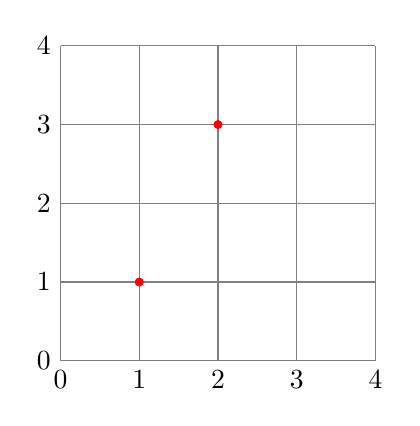
\begin{tikzpicture}
\draw[color=gray, thin] (0,0) grid (4,4);
\foreach \x in {0,...,4}{
\node[anchor=east] at (0,\x){\x};
\node[anchor=north] at (\x,0){\x};}
\draw[color=red, fill] (1,1) circle (0.05);
\draw[color=red, fill] (2,3) circle (0.05);
\elload(1,1)(2,3);
\end{tikzpicture}
\end{minipage}
\begin{minipage}{0.45\textwidth}
\color{mygray}
\verb+\begin{tikzpicture}+
\verb+\draw[color=gray, thin] (0,0) grid (4,4);+
\verb+\foreach \x in {0,...,4}{+
\verb+\node[anchor=east] at (0,\x){\x};+
\verb+\node[anchor=north] at (\x,0){\x};}+
\verb+\draw[color=red, fill] (1,1) circle (0.05);+
\verb+\draw[color=red, fill] (2,3) circle (0.05);+
\color{black}
\verb+\elload(1,1)(2,3);+
\color{mygray}
\verb+\end{tikzpicture}+
\end{minipage}
\end{examplebox}
%
\newpage
\paragraph{Machine}  \ \color{myblue}
\verb+\machine(coordinate1)(coordinate2);+ \color{black}

\begin{examplebox}

\begin{tikzpicture}
\node[anchor=west] at (6,0){\verb+\machine(3,0)(0,0);+};
\machine(0,0)(3,0);
\end{tikzpicture}
\end{examplebox}
\ \\
The machine symbol is based on a simple circular shape with a centred node text. The node text can be accessed either by the option \verb+mode+ to use one of the predefined entries or by the option \verb+text+ to set the entry manually. 
\begin{small}
\begin{examplebox}
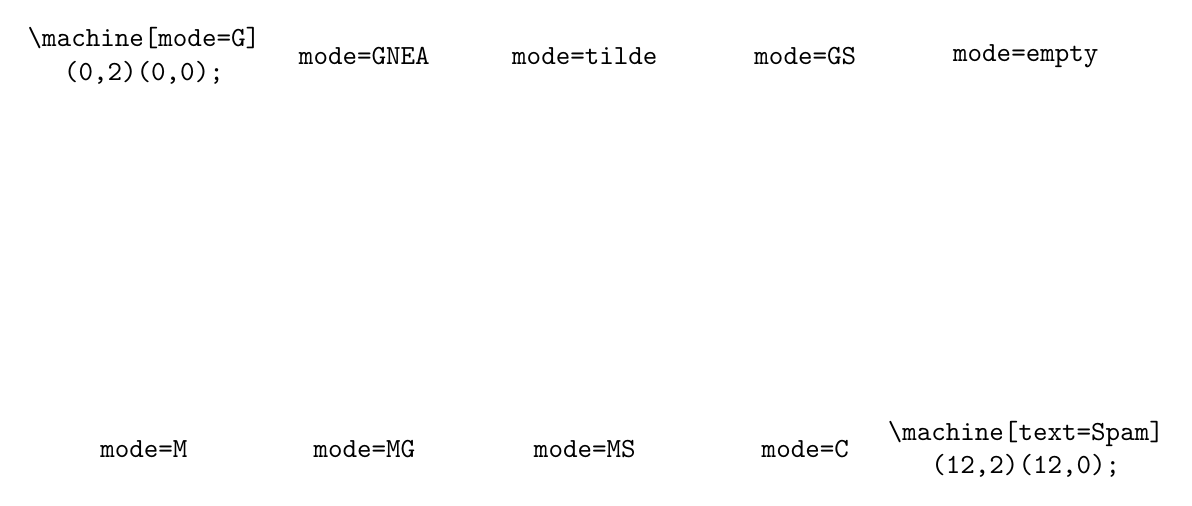
\begin{tikzpicture}
\machine[mode=G]
(0,2)(0,0);
\machine[mode=GNEA](2.8,2)(2.8,0);
\machine[mode=tilde](5.6,2)(5.6,0);
\machine[mode=GS](8.4,2)(8.4,0);
\machine[mode=empty](11.2,2)(11.2,0);
\node[align = center, inner sep = 0pt] at (0,2.75){\verb+\machine[mode=G]+ \\\verb+(0,2)(0,0);+};
\node at (2.8,2.75){\texttt{mode=GNEA}};
\node at (5.6,2.75){\texttt{mode=tilde}};
\node at (8.4,2.75){\texttt{mode=GS}};
\node at (11.2,2.75){\texttt{mode=empty}};
\begin{scope}[yshift=-5cm]
\machine[mode=M](0,2)(0,0);
\machine[mode=MG](2.8,2)(2.8,0);
\machine[mode=MS](5.6,2)(5.6,0);
\machine[mode=C](8.4,2)(8.4,0);
\machine[text=Spam](11.2,2)(11.2,0);
\node at (0,2.75){\texttt{mode=M}};
\node at (2.8,2.75){\texttt{mode=MG}};
\node at (5.6,2.75){\texttt{mode=MS}};
\node at (8.4,2.75){\texttt{mode=C}};
\node[align = center, inner sep = 0pt] at (11.2,2.75){\verb+\machine[text=Spam]+ \\\verb+(12,2)(12,0);+};
\end{scope}
\end{tikzpicture}
\end{examplebox}
\end{small}
\ \\
%
The rotational behaviour of the machines is somewhat different from other commands, to ensure a defined orientation of the node text.
\begin{figure}[H]
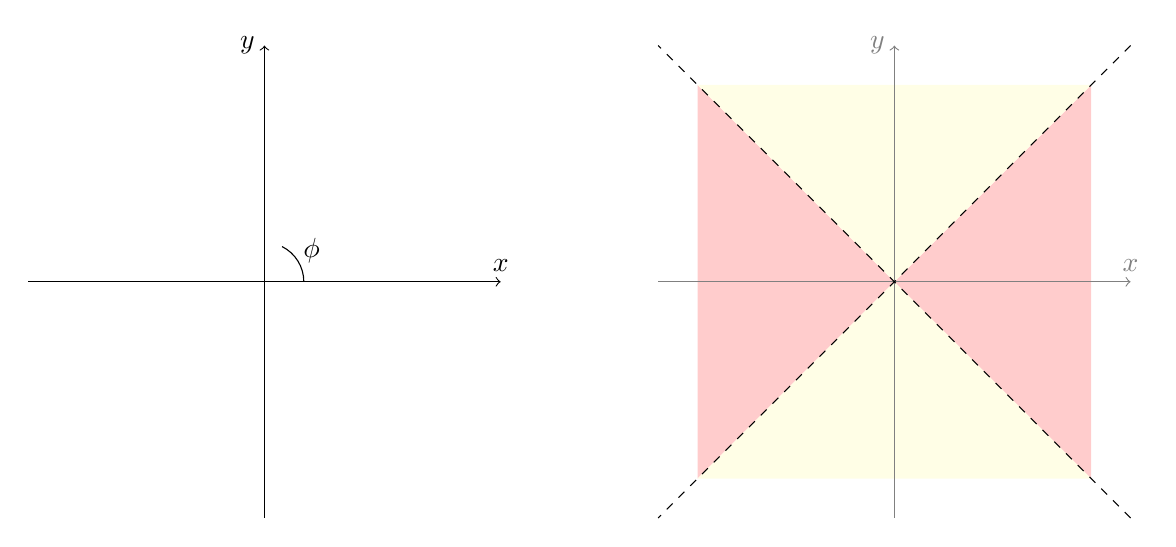
\begin{tikzpicture}
\begin{scope}[]
\node (a) at (1,2){};
\node (b) at (0,0){};
\node (c) at (1,0){};
\draw  pic [ draw] {angle=c--b--a};
\node at (0.6,0.4){$\phi$};
\node[anchor=south] at (3,0){$x$};
\node[anchor=east] at (0,3){$y$};
\draw[,->](-3,0)--(3,0);
\draw[,<-](0,3)--(0,-3);
\machine(0,0)(1,2);
\end{scope}
\begin{scope}[shift={(8,0)}]
\fill[color=red!20!white](0,0)--(2.5,2.5)--(2.5,-2.5)--(0,0);
\fill[color=red!20!white](0,0)--(-2.5,2.5)--(-2.5,-2.5)--(0,0);
\fill[color=yellow!10!white](0,0)--(-2.5,2.5)--(2.5,2.5)--(0,0);
\fill[color=yellow!10!white](0,0)--(-2.5,-2.5)--(2.5,-2.5)--(0,0);
\draw[color=gray,->](-3,0)--(3,0);
\draw[color=gray,<-](0,3)--(0,-3);
\draw[dashed](3,3)--(-3,-3);
\draw[dashed](3,-3)--(-3,3);
\node[anchor=south, color=gray] at (3,0){$x$};
\node[anchor=east, color=gray] at (0,3){$y$};
\machine[mode=M](0,0)(2,0);
\machine[mode=M](0,0)(0,2);
\machine[mode=M](0,0)(-2,0);
\machine[mode=M](0,0)(0,-2);
\end{scope}
\end{tikzpicture}
\end{figure}
%
In the above figure, $\phi$ is the angle between the positive $x$-axis and the machine. The regions for the different text orientations are marked on the right hand side. In the yellow regions, where $ 45^{\circ} < \phi \leqslant 135^{\circ}$  and $ 225 ^{\circ} < \phi \leqslant 315 ^{\circ}$, the node content is equally oriented to the text direction. In the red marked regions, $ 0^{\circ} < \phi \leqslant 45^{\circ}$, $ 135^{\circ} < \phi \leqslant 225^{\circ}$ and $ 315^{\circ} < \phi \leqslant 360^{\circ}$ the node text is rotated counter clockwise by $90^{\circ}$. 

\paragraph{Photovoltaic} \ \color{myblue}\verb+\pv(coordinate1)(coordinate2);+\color{black}
\begin{examplebox}
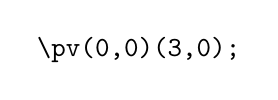
\begin{tikzpicture}
\pv(0,0)(3,0);
\node[anchor=west] at (6,0) {\verb+\pv(0,0)(3,0);+};
\end{tikzpicture}
\end{examplebox}
\paragraph{Load} \ \color{myblue}\verb+\elload(coordinate1)(coordinate2);+\color{black}
\begin{examplebox}
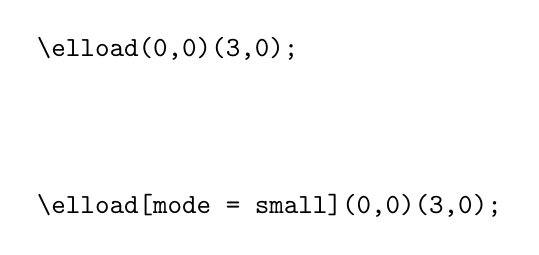
\begin{tikzpicture}
\elload(0,2)(3,2);
\elload[mode=small](0,0)(3,0);
\node[anchor=west] at (6,2) {\verb+\elload(0,0)(3,0);+};
\node[anchor=west] at (6,0) {\verb+\elload[mode = small](0,0)(3,0);+};
\end{tikzpicture}
\end{examplebox}
\paragraph{Ground} \
\color{myblue}{\verb+\ground(coordinate1)(coordinate2);+}\color{black}
\begin{examplebox}

\begin{tikzpicture}
\ground(0,0)(3,0);
\node[anchor=west] at (6,0) {\verb+\ground(0,0)(3,0);+};
\end{tikzpicture}
\end{examplebox}
\paragraph{Grid} \
\color{myblue}\verb+\elgrid(coordinate1)(coordinate2);+\color{black}
\begin{examplebox}
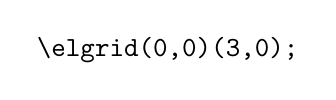
\begin{tikzpicture}
\elgrid(0,0)(3,0);
\node[anchor=west] at (6,0) {\verb+\elgrid(0,0)(3,0);+};
\end{tikzpicture}
\end{examplebox}
\subsection{Bipoles}
Circuit symbols at the center of a line are called bipoles. As monopoles they rely on the basic pattern
\begin{itemize}
        \item[]\color{myblue}{ \verb+\<command>[<optional arguments>](<coordinate1>)(<coordinate2>);+}
\end{itemize}
. Here, the node is placed in the center between \verb+coordinate1+ and \verb+coordinate2+ and rotated accordingly.
\begin{examplebox}
\begin{minipage}{0.45\textwidth}
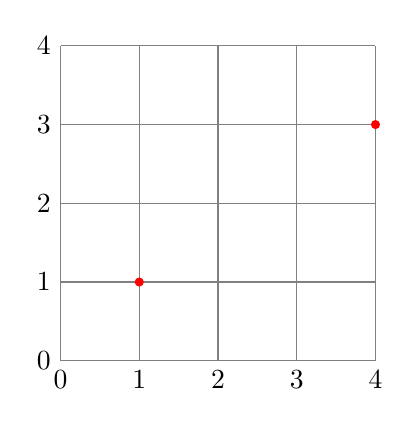
\begin{tikzpicture}
\draw[color=gray, thin] (0,0) grid (4,4);
\foreach \x in {0,...,4}{
\node[anchor=east] at (0,\x){\x};
\node[anchor=north] at (\x,0){\x};}
\draw[color=red, fill] (1,1) circle (0.05);
\draw[color=red, fill] (4,3) circle (0.05);
\trafo(1,1)(4,3);
\end{tikzpicture}
\end{minipage}
\begin{minipage}{0.45\textwidth}
\color{mygray}
\verb+\begin{tikzpicture}+
\verb+\draw[color=gray, thin] (0,0) grid (4,4);+
\verb+\foreach \x in {0,...,4}{+
\verb+\node[anchor=east] at (0,\x){\x};+
\verb+\node[anchor=north] at (\x,0){\x};}+
\verb+\draw[color=red, fill] (1,1) circle (0.05);+
\verb+\draw[color=red, fill] (4,3) circle (0.05);+
\color{black}
\verb+\trafo(1,1)(4,3);+
\color{mygray}
\verb+\end{tikzpicture}+
\end{minipage}
\end{examplebox}
\newpage
\subsubsection{Transformer} 
\label{sec:Trafo}
\begin{itemize}
\item[]\color{myblue}\verb+\trafo(coordinate1)(coordinate1);+
\end{itemize}
The transformer command is treated separately since it is provided with some additional options: three phase transformer connection, neutral point earthing and two color mode. 
First of all, there are some additional transformer variations besides the default shape:
 
\begin{examplebox}
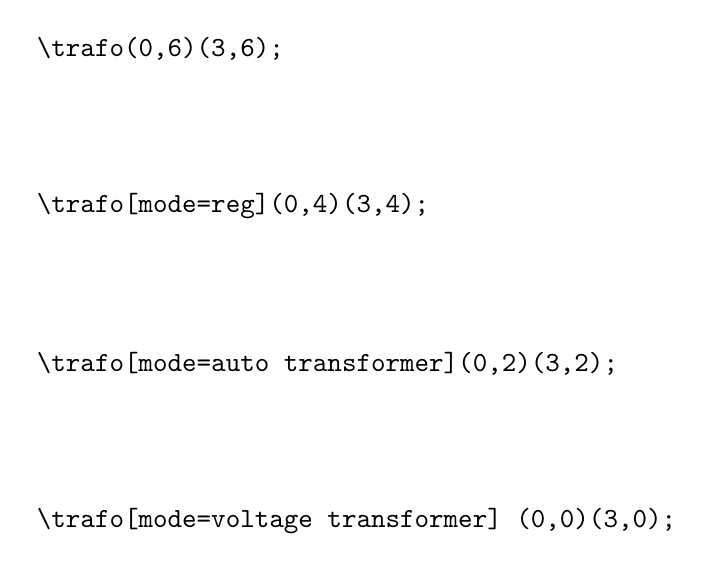
\begin{tikzpicture}
\trafo(0,6)(3,6);
\trafo[mode=reg](0,4)(3,4);
\trafo[mode=auto transformer](0,2)(3,2);
\trafo[mode=voltage transformer] (0,0)(3,0);
\node[anchor=west] at (5,6){\verb+\trafo(0,6)(3,6);+};
\node[anchor=west] at (5,4){\verb+\trafo[mode=reg](0,4)(3,4);+};
\node[anchor=west] at (5,2){\verb+\trafo[mode=auto transformer](0,2)(3,2);+};
\node[anchor=west] at (5,0){\verb+\trafo[mode=voltage transformer] (0,0)(3,0);+};
\end{tikzpicture}
\end{examplebox}
The following options are created to the simple default transformer shape and might look weird in combination with different \verb+modes+ (but feel free to try).
\paragraph{Three phase transformer connection}
Symbols for the three standard three phase transformer connections are defined as node shapes:\\[3pt]
\begin{tikzpicture}
\node[draw, sltrafotriangle] at (0,0){};
\node[draw, sltrafostar] at (5,0){};
\node[draw, sltrafozigzag] at (10,0){};
\node[align=center, inner sep = 0pt] at (0,0.75){\verb+\node[draw, sltrafotriangle]+\\\verb+at (0,0){};+};
\node at (5,0.75){\texttt{sltrafostar}};
\node at (10,0.75){\texttt{sltrafozigzag}};
\end{tikzpicture}
\\ \ \\
They can either be used as shown above as nodes or used within the transformer command with the keyword \verb+group+, followed by a two letters. The first indicates the side of the trafo, which is next to the first coordinate, the letter represents the side next to the  second coordinate. The letters are coded as follows: \\ \ \\[-3mm]
%\begin{table}[H]
\begin{center}
\begin{tabular}{cc}
\texttt{x} = no symbol\hspace{0.75cm} &
\texttt{d} = $\Delta$ - connection\hspace{0.75cm} \\
\texttt{s} = star - connection\hspace{0.75cm} &
\texttt{z} = zigzag - connection \\
\end{tabular}
\end{center}
%\end{table}
\begin{SaveVerbatim}{xd}
\trafo[group=xd](0,2)(4,2);
\end{SaveVerbatim}
\begin{SaveVerbatim}{xx}
\trafo[group=xx](0,0)(4,0);
\end{SaveVerbatim}
\vspace{0.5cm}%\\ \ \\
\begin{examplebox}
\resizebox{\textwidth}{!}{
\begin{tikzpicture}
\trafo[group=xz](0,00)(4,00);
\trafo[group=xs](0,02.5)(4,02.5);
\trafo[group=xd](0,05)(4,05);
\trafo[group=xx](0,07.5)(4,07.5);
\node at (2,0.75){\texttt{group = xz}};
\node at (2,3.25){\texttt{group = xs}};
\node at (2,5.75){\BUseVerbatim{xd}};
\node[align = center] at (2,8.25){\BUseVerbatim{xx}};
\begin{scope}[xshift=5cm,yshift=0cm]
\trafo[group=dz](0,00)(4,00);
\trafo[group=ds](0,02.5)(4,02.5);
\trafo[group=dd](0,05)(4,05);
\trafo[group=dx](0,07.5)(4,07.5);
\node at (2,0.75){\texttt{group = dz}};
\node at (2,3.25){\texttt{group = ds}};
\node at (2,5.75){\texttt{group = dd}};
\node at (2,8.25){\texttt{group = dx}};
\end{scope}
\begin{scope}[xshift=10cm,yshift=0cm]
\trafo[group=sz](0,00)(4,00);
\trafo[group=ss](0,02.5)(4,02.5);
\trafo[group=sd](0,05)(4,05);
\trafo[group=sx](0,07.5)(4,07.5);
\node at (2,0.75){\texttt{group = sz}};
\node at (2,3.25){\texttt{group = ss}};
\node at (2,5.75){\texttt{group = sd}};
\node at (2,8.25){\texttt{group = sx}};
\end{scope}
\begin{scope}[xshift=15cm,yshift=0cm]
\trafo[group=zz](0,00)(4,00);
\trafo[group=zs](0,02.5)(4,02.5);
\trafo[group=zd](0,05)(4,05);
\trafo[group=zx](0,07.5)(4,07.5);
\node at (2,0.75){\texttt{group = zz}};
\node at (2,3.25){\texttt{group = zs}};
\node at (2,5.75){\texttt{group = zd}};
\node at (2,8.25){\texttt{group = zx}};
\end{scope}
\end{tikzpicture}}
\end{examplebox}
\\ \ \\
\paragraph{Neutral point earthing} 
Six variations of neutral point earthing drawings are available. They can be drawn at the transformer side next to the first coordinate using the key \verb+npe first+. The neutral point earthing of the second transformer half can be drawn with the option \verb+npe second+. Both keys can be handled equally - here demonstrated for \verb+npe first+.
\begin{examplebox}
\begin{tikzpicture}
\trafo[group=ss, npe first=sRL](0,0)(4,0);
\trafo[group=ss, npe first=RL](5,0)(9,0);
\trafo[group=ss, npe first=L](10,0)(14,0);
\trafo[group=ss, npe first=R](0,4)(4,4);
\trafo[group=ss, npe first=o](5,4)(9,4);
\trafo[group=ss, npe first=S](10,4)(14,4);
\node at (2,0.75){\texttt{npe first = sRL}};
\node at (7,0.75){\texttt{npe first = RL}};
\node at (12,0.75){\texttt{npe first = L}};
\node[align = center] at (2,5){\verb+\trafo[group=ss, npe first=R]+ \\ \verb+(0,4)(4,4);+};
\node at (7,4.75){\texttt{npe first = o}};
\node at (12,4.75){\texttt{npe first = S}};
\end{tikzpicture}
\end{examplebox}
\begin{examplebox}
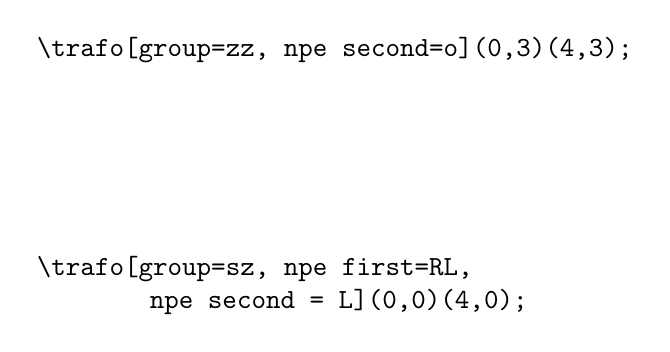
\begin{tikzpicture}
%\begin{scope}[yshift = -7cm]
\trafo[group=zz, npe second=o](0,3)(4,3);
\trafo[group=sz, npe first=RL, npe second = L](0,0)(4,0);
\node[anchor = west] at (4.5,3){\verb+\trafo[group=zz, npe second=o](0,3)(4,3);+};
\node[anchor = west, align = left] at (4.5,0){\verb+\trafo[group=sz, npe first=RL,+\\\hspace{1.25cm}\verb+ npe second = L](0,0)(4,0);+};
%\end{scope}
\end{tikzpicture}
\end{examplebox}
\paragraph{Debug mode}
The \verb+debug+ option of the transformer command prints the coordinates of the point in the transformer circles, where the transformer connections or neutral point earthing are anchored. It can e.g. be used for further neutral point and transformer connection customization.
\begin{examplebox}
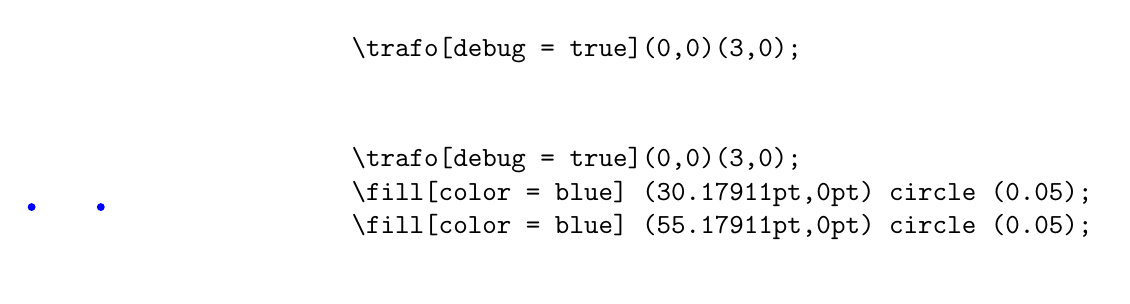
\begin{tikzpicture}
\trafo[debug = true](0,2)(3,2);
\node[anchor = west] at (5,2){\verb+\trafo[debug = true](0,0)(3,0);+};
\trafo[debug = true](0,0)(3,0);
\fill[color = blue] (30.17911pt,0pt) circle (0.05)
                     (55.17911pt,0pt) circle (0.05);   
\node[anchor = west, align = left] at (5,0){\verb+\trafo[debug = true](0,0)(3,0);+\\
\verb+\fill[color = blue] (30.17911pt,0pt) circle (0.05);+\\
\verb+\fill[color = blue] (55.17911pt,0pt) circle (0.05);+\\
};
\end{tikzpicture}
\end{examplebox}
\paragraph{Two colored transformer } In the current version, the two colored transformer option is only defined for the default transformer shape and cannot be combined with neutral point earthing or transformer connections. It can be switched on with the option \verb+two colored+. The colors can then be passed to the command with the keys \verb+first color+ and \verb+second color+. If the colors aren't defined, the current active color is used.
\begin{examplebox}
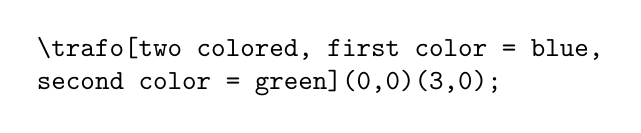
\begin{tikzpicture}
\trafo[two colored, first color = blue, second color = green](0,0)(3,0);
\node[anchor=west, align = left] at (6,0){\verb+\trafo[two colored, first color = blue,+\\\verb+second color = green](0,0)(3,0);+};
\end{tikzpicture}
\end{examplebox}
\subsubsection{More bipoles}
\paragraph{Inverter} \ \color{myblue}
\verb+\inverter(coordinate1)(coordinate2);+\color{black}
\begin{examplebox}
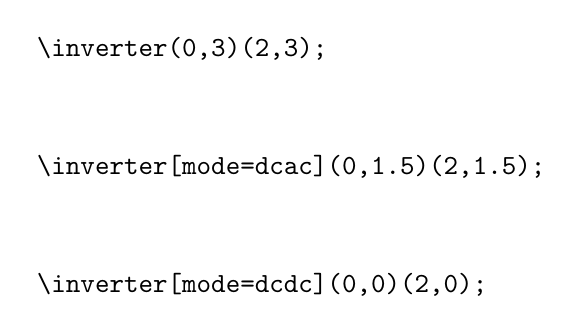
\begin{tikzpicture}
\inverter(0,3)(2,3);
\inverter[mode=dcac](0,1.5)(2,1.5);
\inverter[mode=dcdc](0,0)(2,0);
\node[anchor=west] at (5,3){\verb+\inverter(0,3)(2,3);+};
\node[anchor=west] at (5,1.5){\verb+\inverter[mode=dcac](0,1.5)(2,1.5);+};
\node[anchor=west] at (5,0){\verb+\inverter[mode=dcdc](0,0)(2,0);+};
\end{tikzpicture}
\end{examplebox}
\paragraph{Resistor} \ \color{myblue}
\verb+\resistor(coordinate1)(coordinate2);+ \color{black}
\begin{examplebox}
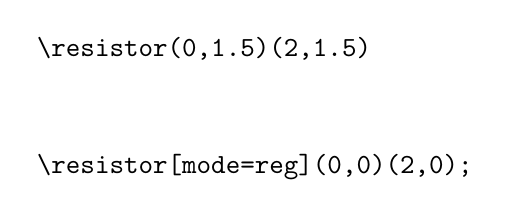
\begin{tikzpicture}
\resistor(0,1.5)(2,1.5);
\resistor[mode=reg](0,0)(2,0);
\node[anchor=west] at (5,1.5){\verb+\resistor(0,1.5)(2,1.5)+};
\node[anchor=west] at (5,0){\verb+\resistor[mode=reg](0,0)(2,0);+};
\end{tikzpicture}
\end{examplebox}
\paragraph{Capacitor} \ \color{myblue} 
\verb+\capacitor(coordinate1)(coordinate2);+ \color{black}
\begin{examplebox}
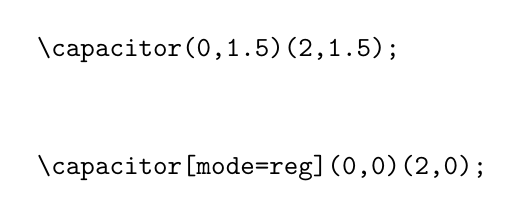
\begin{tikzpicture}
\capacitor(0,1.5)(2,1.5);
\capacitor[mode=reg](0,0)(2,0);
\node[anchor=west] at (5,1.5){\verb+\capacitor(0,1.5)(2,1.5);+};
\node[anchor=west] at (5,0){\verb+\capacitor[mode=reg](0,0)(2,0);+};
\end{tikzpicture}
\end{examplebox}
\paragraph{Switch} \ \color{myblue} 
\verb+\switch(coordinate1)(coordinate2);+ \color{black}
\begin{examplebox}
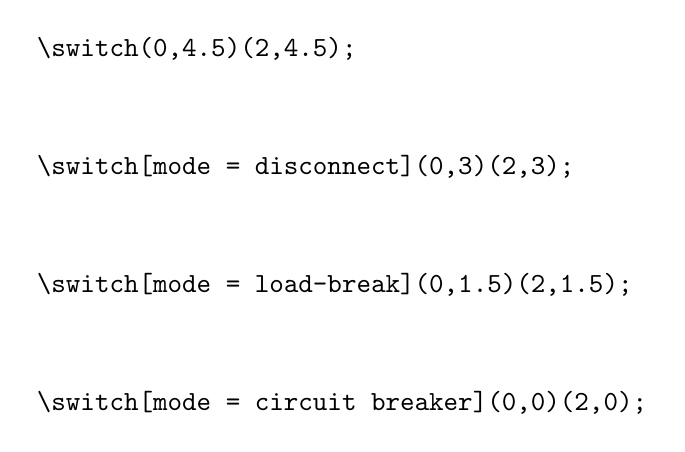
\begin{tikzpicture}
\switch(0,4.5)(2,4.5);
\switch[mode = disconnect](0,3)(2,3);
\switch[mode = load-break](0,1.5)(2,1.5);
\switch[mode = circuit breaker](0,0)(2,0);
\node[anchor=west] at (5, 0)  {\verb+\switch[mode = circuit breaker](0,0)(2,0);+};
\node[anchor=west] at (5, 1.5){\verb+\switch[mode = load-break](0,1.5)(2,1.5);+};
\node[anchor=west] at (5,3)   {\verb+\switch[mode = disconnect](0,3)(2,3);+};
\node[anchor=west] at (5,4.5) {\verb+\switch(0,4.5)(2,4.5);+}; 
\end{tikzpicture}
\end{examplebox}
\paragraph{Reactor} \ \color{myblue}  
\verb+\reactor(coordinate1)(coordinate2);+ \color{black}
\begin{examplebox}
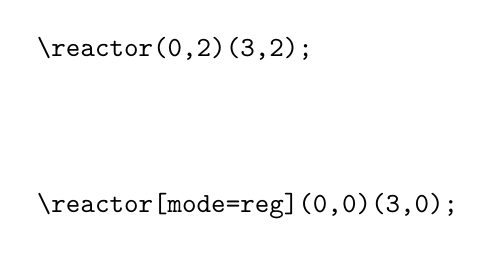
\begin{tikzpicture}
\reactor(0,2)(3,2);
\reactor[mode=reg](0,0)(3,0);
\node[anchor=west] at (5,0){\verb+\reactor[mode=reg](0,0)(3,0);+};
\node[anchor=west] at (5,2){\verb+\reactor(0,2)(3,2);+};
\end{tikzpicture}
\end{examplebox}
\paragraph{Inductance} \ \color{myblue}
\verb+\reactor(coordinate1)(coordinate2);+ \color{black}
\begin{examplebox}
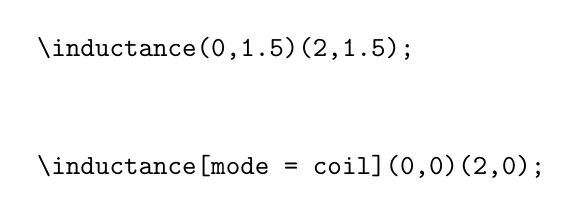
\begin{tikzpicture}
\inductance(0,1.5)(2,1.5);
\inductance[mode = coil](0,0)(2,0);
\node[anchor=west] at (5,0){\verb+\inductance[mode = coil](0,0)(2,0);+};
\node[anchor=west] at (5,1.5){\verb+\inductance(0,1.5)(2,1.5);+};
\end{tikzpicture}
\end{examplebox}
\paragraph{Three phase line} \ \color{myblue}
\verb+\linetp(coordinate1)(coordinate2);+ \color{black}
\begin{examplebox}
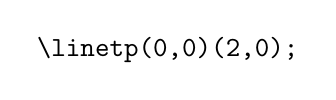
\begin{tikzpicture}
\linetp(0,0)(2,0);
\node[anchor=west] at (5,0){\verb+\linetp(0,0)(2,0);+};
\end{tikzpicture}
\end{examplebox}
\newpage
\subsection{Shapes}
Besides the shapes used in the commands, the following shapes are defined:
\begin{examplebox}
\begin{tikzpicture}
\node[draw,fault] at (0,4){};
\node[draw,currenttransformer] at (0,2){};
\draw(0,1)--(0,0);
\node[draw,currenttransformer] at (0,0.5){};
\node[anchor=west] at (1.5,4){\verb+\node[draw,fault] at (0,4){};+};
\node[anchor=west] at (1.5,2){\verb+\node[draw,currenttransformer] at (0,2){};+};
\node[anchor=west, align=left] at (1.5,0.5){\verb+\node[draw,currenttransformer] at (0,0.5){};+ \\ \verb+\draw(0,1)--(0,0);+};
\end{tikzpicture}
\end{examplebox}
In the table below, the identifiers for shapes used for drawing commands are listed. They can also separately be drawn as nodes. The identifiers are prefixed with "sl" (for single-line), to avoid internal errors.
\begin{table}[h]
\centering
 \setlength{\tabcolsep}{1cm}
\begin{tabular}{lll}
\toprule
\toprule
Command & Mode & Shape identifier\\
\midrule
\verb+\machine+        & all modes             & slcircle      \\
\verb+\pv+              &                       & slpv          \\
\verb+\load+            &                       & slload                \\
\verb+\ground+  &                       & slground      \\
\verb+\elgrid+  &                       & slgrid                \\
\verb+\trafo+   & default       & sltrafo       \\      
                                & \verb+reg+            & slregtrafo \\
                                & \verb+autransformer+          & slautotransformer \\
                            & two colored transformer  & sltwocoloredtrafo\\
                                & \verb+voltage transformer+    &slvoltagetransformer\\
\verb+\inverter+        & default       & sldcac                \\
                                & \verb+acdc+           & slacdc                \\
                                & \verb+dcdc+           & sldcdc                \\
\verb+\resistor+        & default       & slresistor \\
                                & \verb+reg+                    & slregresistor \\
\verb+\capacitor+       & default       & slcapacitor   \\
                                        & \verb+reg+                    & slregcapacitor \\
\verb+\switch+  & default       & slswitch      \\
                                & \verb+circuit breaker+        & slcircbreaker \\
                                & \verb+load-break+     & slloadbreakswitch     \\
                                & \verb+disconnect+     & sldisconswitch        \\
\verb+\reactor+         & default       & slreactor     \\
                                & \verb+reg+                    & slregreactor \\
\verb+\inductance+      & default       & slimpedance   \\
                                & \verb+coil+           & slinductance  \\
\verb+\linetp+  & default       & sllinetp      \\ 
\bottomrule
\bottomrule
\end{tabular}
\end{table}
\pagebreak
\subsection{Bus bar}
\begin{itemize}
\item[]\color{myblue}\verb+\busbar(coordinate 1)(coordinate 2);+ 
\end{itemize}
The default line width of bus bars is 0.3*\verb+\elsize+. The bus bar \verb+label+ option defines label text position and orientation. 
\begin{examplebox}

\begin{tikzpicture}
\busbar(0,0)(2,0);
\node at (7,0){\verb+\busbar(0,0)(2,0);+};
\end{tikzpicture}\\ \ \\ \ \\
\begin{minipage}{0.4\textwidth}
\begin{tikzpicture}
\busbar[label = 1-Spam](0,2)(1,2);
\busbar[label = 2-Spam](2.5,2)(1.5,2);
\busbar[label = 3-Spam](1.25,3.25)(1.25,2.25);
\busbar[label = 4-Spam](1.25,0.75)(1.25,1.75);
\end{tikzpicture}
\end{minipage}
\begin{minipage}{0.45\textwidth}
\begin{verbatim}
\busbar[label = 1-Spam](0,2)(1,2);
\busbar[label = 2-Spam](2.5,2)(1.5,2);
\busbar[label = 3-Spam](1.25,3.25)(1.25,2.25);
\busbar[label = 4-Spam](1.25,0.75)(1.25,1.75);
\end{verbatim}
\end{minipage}
\end{examplebox}
\newpage
\section{Options}
\subsection{General options}
\paragraph{Connectors}
Connectors are basically arrow tips, which are used to connect lines and circuit commands. As a consequence, they can be interchanged with other \Tikz based arrows. The connectors are named with a three-letter scheme:% and consist of three elements, so that each of this letters stands for an element of a connector. 
\begin{table}[h]
%\caption{3-letter naming scheme of the connectors.}
\centering
\begin{tabular}{ccc}
First letter & Second letter & Third letter \\
\midrule
\verb+c+ = closed & \verb+c+ = closed & \verb+t+ = arrow points \textbf{to} the connector\\
\verb+o+ = open & \verb+o+ = open& \verb+f+ = arrow points away \textbf{from} the connector\\
\verb+x+ = not existent& \verb+x+ = not existent & \verb+x+ = not existent \\
\end{tabular}
\label{tab:connectornamingscheme}
\end{table}
\begin{examplebox}
\begin{tikzpicture}
\begin{scope}
\draw[cxx-](1.25,3)--(3.25,3);
\draw[ccx-](1.25,2)--(3.25,2);
\draw[cox-](1.25,1)--(3.25,1);
\draw[oxx-](1.25,0)--(3.25,0);
\draw[ocx-](1.25,-1)--(3.25,-1);
\draw[oox-](1.25,-2)--(3.25,-2);
\draw[xcx-](1.25,-3)--(3.25,-3);
\draw[xox-](1.25,-4)--(3.25,-4);
\node at (0,3){\verb+cxx-+};
\node at (0,2){\verb+ccx-+};
\node at (0,1){\verb+cox-+};
\node at (0,0){\verb+oxx-+};
\node at (0,-1){\verb+ocx-+};
\node at (0,-2){\verb+oox-+};
\node at (0,-3){\verb+xcx-+};
\node at (0,-4){\verb+xox-+};
\draw[cxt-](6.5,3)--(8.5,3);
\draw[cct-](6.5,2)--(8.5,2);
\draw[cot-](6.5,1)--(8.5,1);
\draw[oxt-](6.5,0)--(8.5,0);
\draw[oct-](6.5,-1)--(8.5,-1);
\draw[oot-](6.5,-2)--(8.5,-2);
\draw[xct-](6.5,-3)--(8.5,-3);
\draw[xot-](6.5,-4)--(8.5,-4);
\draw[xxt-](6.5,-5)--(8.5,-5);
\node at (5.25,3){\verb+cxt-+};
\node at (5.25,2){\verb+cct-+};
\node at (5.25,1){\verb+cot-+};
\node at (5.25,0){\verb+oxt-+};
\node at (5.25,-1){\verb+oct-+};
\node at (5.25,-2){\verb+oot-+};
\node at (5.25,-3){\verb+xct-+};
\node at (5.25,-4){\verb+xot-+};
\node at (5.25,-5){\verb+xxt-+};
\draw[cxf-](11.75,3)--(13.75,3);
\draw[ccf-](11.75,2)--(13.75,2);
\draw[cof-](11.75,1)--(13.75,1);
\draw[oxf-](11.75,0)--(13.75,0);
\draw[ocf-](11.75,-1)--(13.75,-1);
\draw[oof-](11.75,-2)--(13.75,-2);
\draw[xcf-](11.75,-3)--(13.75,-3);
\draw[xof-](11.75,-4)--(13.75,-4);
\draw[xxf-](11.75,-5)--(13.75,-5);
\node at (10.5,3){\verb+cxf-+};
\node at (10.5,2){\verb+ccf-+};
\node at (10.5,1){\verb+cof-+};
\node at (10.5,0){\verb+oxf-+};
\node at (10.5,-1){\verb+ocf-+};
\node at (10.5,-2){\verb+oof-+};
\node at (10.5,-3){\verb+xcf-+};
\node at (10.5,-4){\verb+xof-+};
\node at (10.5,-5){\verb+xxf-+};
\end{scope}
%\draw[step=1cm,gray,very thin] (0,0) grid (16,7);
\end{tikzpicture}
\end{examplebox}
\begin{examplebox}
\begin{tikzpicture}
\begin{scope}
\draw[ccx-ccx] (0,0)--(2,0);
\inverter[connector=cxx-ccx](0,2)(2,2);
\inverter[connector=ccx-](0,4)(2,4);
\inverter[connector=-ccx](0,6)(2,6);
\node[anchor=west] at (5,0){\verb+\draw[ccx-ccx] (0,0)--(2,0);+};
\node[anchor=west] at (5,2){\verb+\inverter[connector=cxx-ccx](0,0)(2,0);+};
\node[anchor=west] at (5,4){\verb+\inverter[connector=ccx-](0,2)(2,2);+};
\node[anchor=west] at (5,6){\verb+\inverter[connector=-ccx](0,4)(2,4);+};
\end{scope}
\end{tikzpicture}
\end{examplebox}

\newpage
\paragraph{Color} \
%Works for all elements. The circle in the connector is always black in this version and cannot be changed.
\begin{examplebox}
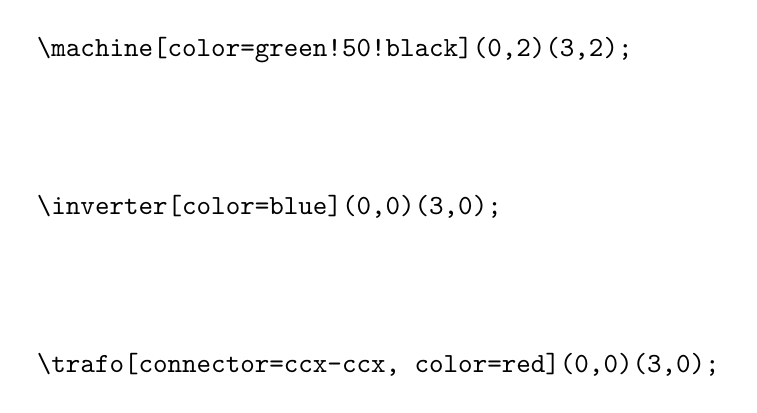
\begin{tikzpicture}
\inverter[color=blue](0,2)(3,2);
\machine[color=green!50!black](0,4)(3,4);
\trafo[connector=ccx-ccx, color=red](0,0)(3,0);
\node[anchor=west] at (5,2){\verb+\inverter[color=blue](0,0)(3,0);+};
\node[anchor=west] at (5,4){\verb+\machine[color=green!50!black](0,2)(3,2);+};
\node[anchor=west] at (5,0){\verb+\trafo[connector=ccx-ccx, color=red](0,0)(3,0);+
};
\end{tikzpicture}
\end{examplebox}
\paragraph{Scale} \
\verb+scale+ is only designed for shape scaling. Line width and connectors can be scaled using the \verb+line width+ key.
\begin{examplebox}
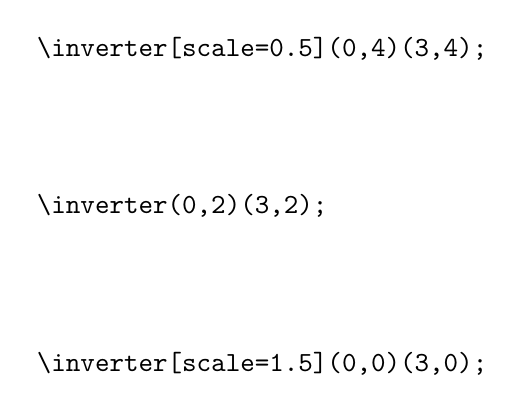
\begin{tikzpicture}
\inverter[scale=0.5](0,4)(3,4);
\inverter(0,2)(3,2);
\inverter[scale=1.5](0,0)(3,0);
\node[anchor=west] at (5,4){\verb+\inverter[scale=0.5](0,4)(3,4);+};
\node[anchor=west] at (5,2){\verb+\inverter(0,2)(3,2);+};
\node[anchor=west] at (5,0){\verb+\inverter[scale=1.5](0,0)(3,0);+};
\end{tikzpicture}
\end{examplebox}
\paragraph{Mirror}\
The shape of the element is mirrored along the axis perpendicular to the drawing axis. 
\begin{examplebox}
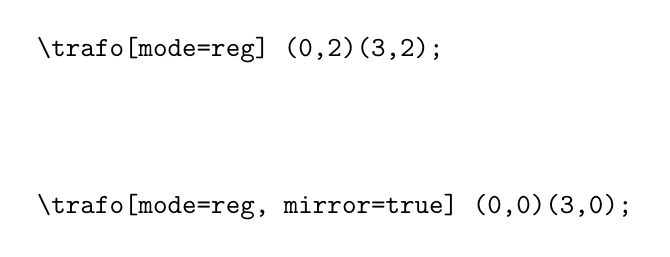
\begin{tikzpicture}
\trafo[mode=reg](0,2)(3,2);
\trafo[mode=reg, mirror=true](0,0)(3,0);
%\trafo[mode=reg](0,0)(0,3);
%\trafo[mode=reg,mirror=true](2,0)(2,3);
%\node[anchor=west] at (5,1.75){\verb+\trafo[mode=reg] (0,0)(3,0);+};
%\node[anchor=west] at (5,1.25){\verb+\trafo[mode=reg, mirror=true] (2,0)(2,3);+};
\node[anchor=west] at (5,2){\verb+\trafo[mode=reg] (0,2)(3,2);+};
\node[anchor=west] at (5,0){\verb+\trafo[mode=reg, mirror=true] (0,0)(3,0);+};
\end{tikzpicture}
\end{examplebox}
\paragraph{Line width} \ 
\begin{examplebox}
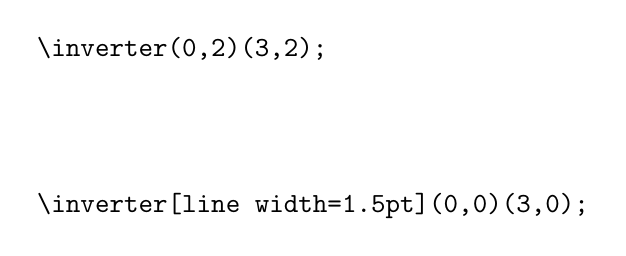
\begin{tikzpicture}
\inverter(0,2)(3,2);
\inverter[line width=1.5pt](0,0)(3,0);
\node[anchor=west] at (5,2){\verb+\inverter(0,2)(3,2);+};
\node[anchor=west] at (5,0){\verb+\inverter[line width=1.5pt](0,0)(3,0);+};
\end{tikzpicture}
\end{examplebox}
\newpage
\subsection{Element size and scaling}
Every shapes is defined using a reference size, called \verb+\elsize+. Changing the \verb+\elsize+ thus changes the size of all shapes defined in the \verb+singleline+ package and should be used carefully.
However, there are some predefined settings for the \verb+elsize+, which can be called globally as package options, e.g. \verb+\usepackage[small]{singleline}+ or local with the commands in the table below.
\begin{table}[H]
\centering
\begin{tabular}{llc}
%\centering
\toprule
\toprule
Command &Package option & \verb+elsize+ \\
\midrule
\verb+\singlelinetiny+ &\verb+tiny+ & 3pt \\
\verb+\singlelinesmall+&\verb+small+ & 4pt \\
\verb+\singlelinenormal+&\verb+normal+ (default) & 5pt \\
\verb+\singlelinetall+&\verb+tall+ & 6pt \\
\verb+\singlelinehuge+&\verb+huge+ & 7pt \\
\bottomrule
\bottomrule
\end{tabular}
\end{table}
\begin{examplebox}
\centering
\begin{tikzpicture}
\renewcommand{\elsize}{6.*0.5pt}
\begin{scope}
\node[align=center] at (1.5,6.5){\verb+\singlelinetiny+\\\verb+tiny+};
\busbar(0,6)(3,6);
\trafo(1.5,6)(1.5,3);
\busbar(0,3)(3,3);
\machine[mode=G](0.5,3)(0.5,1);
\elgrid(2.5,3)(2.5,1);
\end{scope}
\renewcommand{\elsize}{8.*0.5pt}
\begin{scope}[xshift=4cm]
\node[align=center] at (1.5,6.5){\verb+\singlelinesmall+\\\verb+small+};
\busbar(0,6)(3,6);
\trafo(1.5,6)(1.5,3);
\busbar(0,3)(3,3);
\machine[mode=G](0.5,3)(0.5,1);
\elgrid(2.5,3)(2.5,1);
\end{scope}
\renewcommand{\elsize}{10.*0.5pt}
\begin{scope}[xshift=8cm]
\node[align = center] at (1.5,6.5){\verb+\singlelinenormal+\\\verb+normal+};
\busbar(0,6)(3,6);
\trafo(1.5,6)(1.5,3);
\busbar(0,3)(3,3);
\machine[mode=G](0.5,3)(0.5,1);
\elgrid(2.5,3)(2.5,1);
\end{scope}
\renewcommand{\elsize}{12.*0.5pt}
\begin{scope}[yshift=-7.5cm,xshift=2cm]
\node[align=center] at (1.5,6.5){\verb+\singlelinetall+\\\verb+tall+};
\busbar(0,6)(3,6);
\trafo(1.5,6)(1.5,3);
\busbar(0,3)(3,3);
\machine[mode=G](0.5,3)(0.5,1);
\elgrid(2.5,3)(2.5,1);
\end{scope}
\renewcommand{\elsize}{14.*0.5pt}
\begin{scope}[yshift=-7.5cm,xshift=6cm]
\node[align=center] at (1.5,6.5){\verb+\singlelinehuge+\\\verb+huge+};
\busbar(0,6)(3,6);
\trafo(1.5,6)(1.5,3);
\busbar(0,3)(3,3);
\machine[mode=G](0.5,3)(0.5,1);
\elgrid(2.5,3)(2.5,1);
\end{scope}
\end{tikzpicture}
\end{examplebox}
\newpage
\section{Examples}
\subsection{9 Bus system} \
\resizebox{0.95\textwidth}{!}{
\centering
\begin{tikzpicture}
%\draw[dashed, color=darkgreen] (-13,0) grid (13,18);
%\foreach \x in {-13,...,13}{
%\node[anchor=north, color=red] at (\x,0){\x};}
%\foreach \x in {0,...,18}{
%\node[anchor=east, color=red] at (0,\x){\x};}
\busbar[label=Bus 1](8,-1)(12,-1);
\busbar[label=Bus 2](0,9)(0,12);
\busbar[label=Bus 3](19,9)(19,12);
\busbar[label=Bus 4](6,3)(14,3);
\busbar[label=Bus 5](4,6)(7,6);
\busbar[label=Bus 6](12,6)(15,6);
\busbar[label=Bus 7](4,9)(4,13);
\busbar[label=Bus 8](10,10)(10,14);
\busbar[label=Bus 9](15,9)(15,13);
\machine[connector=ccx-,mode=G](10,-1)($(10,-1)-(0,2)$);
\machine[connector=ccx-, mode=G](0,11)($(0,11)-(2,0)$);
\elload[connector=ccx-](4.5,6)($(4.5,6)-(0,2)$);
\elload[connector=ccx-](4,10)($(4,10)-(2,0)$);
\elload[connector=ccx-](10,13)($(10,13)+(2,0)$);
\elgrid[connector=ccx-](19,10)($(19,10)+(2,0)$);
\elgrid[connector=ccx-](10,11)($(10,11)-(2,0)$);
\trafo[connector=cct-ccx](10,-1)(10,3);
\trafo[connector=cct-ccx](4,11)(0,11);
\trafo[connector=cct-ccx](15,11)(19,11);
%
\draw[cct-ccx](6.5,6)--(6.5,3); 
\draw[ccf-ccf](13.5,6)--(13.5,3); 
\draw[ccx-cct](4,11)-|(6,6); 
\draw[ccx-cct](15,11)-|(13.5,6);
\draw[ccx-cct](4,12)--(10,12); 
\draw[cct-ccx](10,12)--(15,12); 
\end{tikzpicture}}
\begin{small}
\begin{verbatim}
\begin{tikzpicture}
%
\busbar[label=Bus 1](8,-1)(12,-1);
\busbar[label=Bus 2](0,9)(0,12);
\busbar[label=Bus 3](19,9)(19,12);
\busbar[label=Bus 4](6,3)(14,3);
\busbar[label=Bus 5](4,6)(7,6);
\busbar[label=Bus 6](12,6)(15,6);
\busbar[label=Bus 7](4,9)(4,13);
\busbar[label=Bus 8](10,10)(10,14);
\busbar[label=Bus 9](15,9)(15,13);
%
\machine[connector=ccx-,mode=G](10,-1)($(10,-1)-(0,2)$);
\machine[connector=ccx-, mode=G](0,11)($(0,11)-(2,0)$);
\elload[connector=ccx-](4.5,6)($(4.5,6)-(0,2)$);
\elload[connector=ccx-](4,10)($(4,10)-(2,0)$);
\elload[connector=ccx-](10,13)($(10,13)+(2,0)$);
\elgrid[connector=ccx-](19,10)($(19,10)+(2,0)$);
\elgrid[connector=ccx-](10,11)($(10,11)-(2,0)$);
\trafo[connector=cct-ccx](10,-1)(10,3);
\trafo[connector=cct-ccx](4,11)(0,11);
\trafo[connector=cct-ccx](15,11)(19,11);
\draw[cct-ccx](6.5,6)--(6.5,3); 
\draw[ccf-ccf](13.5,6)--(13.5,3); 
\draw[ccx-cct](4,11)-|(6,6); 
\draw[ccx-cct](15,11)-|(13.5,6);
\draw[ccx-cct](4,12)--(10,12); 
\draw[cct-ccx](10,12)--(15,12); 
%
\end{tikzpicture}
\end{verbatim}
\end{small}
\subsection{Shape orientation}
Sometimes, the default orientation of a circuit symbol in a command might not be ideal. Symbols can simply be rotated by 180 degrees by interchanging the first and second coordinate of the command. In combination with the previously mentioned mirror option, the desired orientation should be possible.
\begin{examplebox}
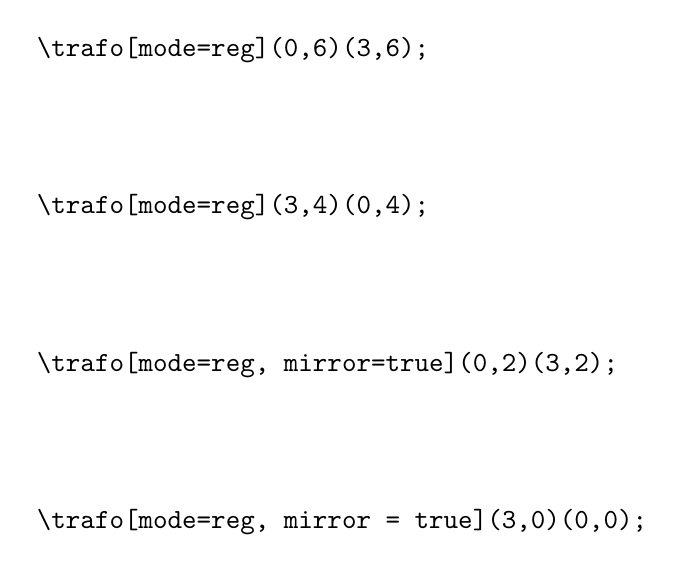
\begin{tikzpicture}
\trafo[mode=reg](0,6)(3,6);
\trafo[mode=reg](3,4)(0,4);
\trafo[mode=reg, mirror=true](0,2)(3,2);
\trafo[mode=reg, mirror = true](3,0)(0,0);
\node[anchor=west] at (5,6){\verb+\trafo[mode=reg](0,6)(3,6);+};
\node[anchor=west] at (5,4){\verb+\trafo[mode=reg](3,4)(0,4);+};
\node[anchor=west] at (5,2){\verb+\trafo[mode=reg, mirror=true](0,2)(3,2);+};
\node[anchor=west] at (5,0){\verb+\trafo[mode=reg, mirror = true](3,0)(0,0);+};
\end{tikzpicture}
\end{examplebox}
\section{Advanced settings }
\subsection{Defining global options}
The \verb+singeline+ package uses, as \Tikz, heavily the \verb+pgfkey+ mechanism. The default values for commands and their optional arguments are stored in a pgfkey tree. By altering the key values, options can be set globally for the entire document, or if used in some sort of scoping environment, for a section. Detailed information about the pgf keys can be found in the pgf documentation. 
For \verb+singlelinetikz+ defined keys can be found in the next section. The values of the keys can be manipulated in the easiest way with \verb+\pgfkeys{}+.
\paragraph{Example} \ \\
\begin{examplebox}
\begin{minipage}{0.25\textwidth}
\begin{tikzpicture}
\switch(0,4.5)(2,4.5);
\pgfkeys{/tikz/singleline/bipoles/switch/mode=load-break}
\switch(0,3)(2,3);
\pgfkeys{/tikz/singleline/bipoles/switch/color=blue}
\switch(0,1.5)(2,1.5);
\pgfkeys{/tikz/singleline/bipoles/switch/mirror=true}
\switch(0,0)(2,0);
\end{tikzpicture}
\end{minipage}
\begin{minipage}{0.55\textwidth}
\begin{verbatim}
\switch(0,4.5)(2,4.5);
\pgfkeys{/tikz/singleline/bipoles/switch/mode=load-break}
\switch(0,3)(2,3);
\pgfkeys{/tikz/singleline/bipoles/switch/color=blue}
\switch(0,1.5)(2,1.5);
\pgfkeys{/tikz/singleline/bipoles/switch/mirror=true}
\switch(0,0)(2,0);
\end{verbatim}
\end{minipage}
\end{examplebox}
\twocolumn[
\subsection{Pgfkey tree}]
\begin{footnotesize}
%\paragraph{Singleline Settings:}
\paragraph{Machine}
\begin{verbatim}
/tikz/singleline/monopoles/machine
/tikz/singleline/monopoles/machine/color
/tikz/singleline/monopoles/machine/scale
/tikz/singleline/monopoles/machine/line width
/tikz/singleline/monopoles/machine/label
/tikz/singleline/monopoles/machine/mode
/tikz/singleline/monopoles/machine/text
/tikz/singleline/monopoles/machine/shape
/tikz/singleline/monopoles/machine/connector
/tikz/singleline/monopoles/machine/leftconnector
/tikz/singleline/monopoles/machine/rightconnector
\end{verbatim}
\paragraph{Photovoltaic}
\begin{verbatim}
/tikz/singleline/monopoles/pv
/tikz/singleline/monopoles/pv/color
/tikz/singleline/monopoles/pv/scale
/tikz/singleline/monopoles/pv/line width
/tikz/singleline/monopoles/pv/label
/tikz/singleline/monopoles/pv/shape
/tikz/singleline/monopoles/pv/connector
/tikz/singleline/monopoles/pv/leftconnector
/tikz/singleline/monopoles/pv/rightconnector
\end{verbatim}
\paragraph{Load}
\begin{verbatim}
/tikz/singleline/monopoles/load
/tikz/singleline/monopoles/load/color
/tikz/singleline/monopoles/load/scale
/tikz/singleline/monopoles/load/line width
/tikz/singleline/monopoles/load/label
/tikz/singleline/monopoles/load/mode
/tikz/singleline/monopoles/load/shape
/tikz/singleline/monopoles/load/connector
/tikz/singleline/monopoles/load/leftconnector
/tikz/singleline/monopoles/load/rightconnector
\end{verbatim}
\paragraph{Ground}
\begin{verbatim}
/tikz/singleline/monopoles/ground
/tikz/singleline/monopoles/ground/color
/tikz/singleline/monopoles/ground/scale
/tikz/singleline/monopoles/ground/line width
/tikz/singleline/monopoles/ground/label
/tikz/singleline/monopoles/ground/shape
/tikz/singleline/monopoles/ground/connector
/tikz/singleline/monopoles/ground/leftconnector
/tikz/singleline/monopoles/ground/rightconnector
\end{verbatim}
\paragraph{Grid}
\begin{verbatim}
/tikz/singleline/monopoles/grid
/tikz/singleline/monopoles/grid/color
/tikz/singleline/monopoles/grid/scale
/tikz/singleline/monopoles/grid/line width
/tikz/singleline/monopoles/grid/label
/tikz/singleline/monopoles/grid/shape
/tikz/singleline/monopoles/grid/connector
/tikz/singleline/monopoles/grid/leftconnector
/tikz/singleline/monopoles/grid/rightconnector
\end{verbatim}
\paragraph{Transformer}
\begin{verbatim}
/tikz/singleline/bipoles/trafo
/tikz/singleline/bipoles/trafo/color
/tikz/singleline/bipoles/trafo/scale
/tikz/singleline/bipoles/trafo/line width
/tikz/singleline/bipoles/trafo/label
/tikz/singleline/bipoles/trafo/shape
/tikz/singleline/bipoles/trafo/connector
/tikz/singleline/bipoles/trafo/leftconnector
/tikz/singleline/bipoles/trafo/rightconnector
/tikz/singleline/bipoles/trafo/group
/tikz/singleline/bipoles/trafo/group draw
/tikz/singleline/bipoles/trafo/debug
/tikz/singleline/bipoles/trafo/npe first
/tikz/singleline/bipoles/trafo/npe draw first
/tikz/singleline/bipoles/trafo/npe second
/tikz/singleline/bipoles/trafo/npe draw second
/tikz/singleline/bipoles/trafo/two colored
/tikz/singleline/bipoles/trafo/first color
/tikz/singleline/bipoles/trafo/second color
\end{verbatim}
\paragraph{Capacitor}
\begin{verbatim}
/tikz/singleline/bipoles/capacitor
/tikz/singleline/bipoles/capacitor/color
/tikz/singleline/bipoles/capacitor/label
/tikz/singleline/bipoles/capacitor/line width
/tikz/singleline/bipoles/capacitor/connector
/tikz/singleline/bipoles/capacitor/leftconnector
/tikz/singleline/bipoles/capacitor/rightconnector
/tikz/singleline/bipoles/capacitor/shape
/tikz/singleline/bipoles/capacitor/scale
/tikz/singleline/bipoles/capacitor/mirror
/tikz/singleline/bipoles/capacitor/mode
\end{verbatim}
\paragraph{Inverter}
\begin{verbatim}
/tikz/singleline/bipoles/inverter
/tikz/singleline/bipoles/inverter/color
/tikz/singleline/bipoles/inverter/label
/tikz/singleline/bipoles/inverter/line width
/tikz/singleline/bipoles/inverter/connector
/tikz/singleline/bipoles/inverter/leftconnector
/tikz/singleline/bipoles/inverter/rightconnector
/tikz/singleline/bipoles/inverter/shape
/tikz/singleline/bipoles/inverter/scale
/tikz/singleline/bipoles/inverter/mirror
/tikz/singleline/bipoles/inverter/mode
\end{verbatim}
\paragraph{Inductance}
\begin{verbatim}
/tikz/singleline/bipoles/inductance
/tikz/singleline/bipoles/inductance/color
/tikz/singleline/bipoles/inductance/label
/tikz/singleline/bipoles/inductance/line width
/tikz/singleline/bipoles/inductance/connector
/tikz/singleline/bipoles/inductance/leftconnector
/tikz/singleline/bipoles/inductance/rightconnector
/tikz/singleline/bipoles/inductance/shape
/tikz/singleline/bipoles/inductance/scale
/tikz/singleline/bipoles/inductance/mirror
/tikz/singleline/bipoles/inductance/mode
\end{verbatim}
\paragraph{Three phase line}
\begin{verbatim}
/tikz/singleline/bipoles/linetp
/tikz/singleline/bipoles/linetp/color
/tikz/singleline/bipoles/linetp/label
/tikz/singleline/bipoles/linetp/line width
/tikz/singleline/bipoles/linetp/connector
/tikz/singleline/bipoles/linetp/leftconnector
/tikz/singleline/bipoles/linetp/rightconnector
/tikz/singleline/bipoles/linetp/shape
/tikz/singleline/bipoles/linetp/scale
/tikz/singleline/bipoles/linetp/mirror
\end{verbatim}
\paragraph{Resistor}
\begin{verbatim}
/tikz/singleline/bipoles/resistor
/tikz/singleline/bipoles/resistor/color
/tikz/singleline/bipoles/resistor/label
/tikz/singleline/bipoles/resistor/line width
/tikz/singleline/bipoles/resistor/connector
/tikz/singleline/bipoles/resistor/leftconnector
/tikz/singleline/bipoles/resistor/rightconnector
/tikz/singleline/bipoles/resistor/shape
/tikz/singleline/bipoles/resistor/scale
/tikz/singleline/bipoles/resistor/mirror
/tikz/singleline/bipoles/resistor/mode
\end{verbatim}
\paragraph{Switch}
\begin{verbatim}
/tikz/singleline/bipoles/switch
/tikz/singleline/bipoles/switch/color
/tikz/singleline/bipoles/switch/label
/tikz/singleline/bipoles/switch/line width
/tikz/singleline/bipoles/switch/connector
/tikz/singleline/bipoles/switch/leftconnector
/tikz/singleline/bipoles/switch/rightconnector
/tikz/singleline/bipoles/switch/shape
/tikz/singleline/bipoles/switch/scale
/tikz/singleline/bipoles/switch/mirror
/tikz/singleline/bipoles/switch/mode
\end{verbatim}
\paragraph{Reactor}
\begin{verbatim}
/tikz/singleline/bipoles/reactor
/tikz/singleline/bipoles/reactor/color
/tikz/singleline/bipoles/reactor/label
/tikz/singleline/bipoles/reactor/line width
/tikz/singleline/bipoles/reactor/connector
/tikz/singleline/bipoles/reactor/leftconnector
/tikz/singleline/bipoles/reactor/rightconnector
/tikz/singleline/bipoles/reactor/shape
/tikz/singleline/bipoles/reactor/scale
/tikz/singleline/bipoles/reactor/mirror
/tikz/singleline/bipoles/reactor/mode
\end{verbatim}
\paragraph{Bus bar}
\begin{verbatim}
/tikz/singleline/busbar/busbar line width
/tikz/singleline/busbar/label
/tikz/singleline/busbar/color
/tikz/singleline/busbar/leftconnector
/tikz/singleline/busbar/rightconnector
/tikz/singleline/busbar/connector
\end{verbatim}
\end{footnotesize}
\onecolumn
\begin{itemize}
\item ...\verb+/color+: Defines drawing color. Default: . 
\item ...\verb+/scale+: Defines scale factor. Default: 1
\item ...\verb+/shape+: Stores the used shape. Default: see section 2.3. 
\item ...\verb+/line width+: Defines line width. Default:  0.4pt.
\item ...\verb+/label+: Sets label. Default: empty
\item ...\verb+mode+: The \verb+mode+ keys are created as \verb+.is choice+- keys. The choice sets the value of the \verb+shape+-key to the corresponding node shape.
\item ...\verb+/trafo/group+: Is an \verb+.is choice+-key, that sets the value of ...\verb+/trafo/group draw+ according to the selected sub-key.
\item ...\verb+/trafo/group draw+: Contains the drawing commands for the transformer three phase connections (see section \ref{sec:Trafo}).
\item ...\verb+/trafo/npe first+: Is an \verb+.is choice+ key, that sets the value of ...\verb+/trafo/npe draw first+
\item ...\verb+/trafo/npe draw first+ stores the drawing commands for the neutral pint earthing on the first transformer half.
\item ...\verb+/trafo/npe second+ and ..\verb+/trafo/npe draw second+: As draw first, but for the second transformer side.
\item ...\verb+/trafo/two colored+ Turns on the two colored mode.
\item ...\verb+/trafo/first color+ and ...\verb+/trafo/second color+ Set colors for two colored transformer mode. Default: .
\item ...\verb+/busbar/busbar line width+: Line width of bus bars. Default: 0.3*\verb+\elsize+.
\item ...\verb+/busbar/label+: Bus bar label. 
\end{itemize}
\onehalfspacing
\subsection{Defining a new drawing command}
Defining new drawing commands with this package is quite simple. Most circuit symbol commands rely on two basic commands, one is used for the definition of monopoles and the other for bipoles.
These commands basically support the "standard " drawing options that have been listed in section 3.1. Commands as \verb+\trafo+ with extended options are defined separately.
The basic commands can be understood as an input mask, that reads the specified information from a previously defined pgf key tree.
Assume, one wants to create a new bipole \verb+\foo+ with a simple round node at the center. The first step is to create the necessary pgf tree and define the default values. For a bipole the following form is required:
\begin{footnotesize}
\begin{verbatim}
\pgfkeysdefargs{/tikz/singleline/bipoles/foo/connector}{#1-#2}{
        \pgfkeys{/tikz/singleline/bipoles/foo/leftconnector=#1-}
        \pgfkeys{/tikz/singleline/bipoles/foo/rightconnector=-#2}}
\pgfkeys{/tikz/singleline/bipoles/foo/.cd,
color/.initial={blue},
label/.initial={},
line width/.initial={2pt},
leftconnector/.initial={},
rightconnector/.initial={},
connector/.initial={ - },
shape/.initial={circle},
scale/.initial={1},
mirror/.initial={false},
mode/.is choice,}
\end{verbatim}
\end{footnotesize}
%
%
Afterwards the command can be defined using the macro
\begin{verbatim} 
\NewDocumentCommand{\foo}{O{}r()r()}{
\SinglelineDefineBipoleCommands[#1]{foo}{#2}{#3}} .
\end{verbatim}
If one appends these lines in the \verb+singleline.sty+ document and reinstalls the package, one should be able to generate this output without errors:
\begin{examplebox}
\begin{minipage}{0.45\textwidth}

\begin{tikzpicture}
%\foo(0,0)(2,0);
\node[draw, circle, line width = 2pt, color = blue] (circle) at (1,0){};
\draw[line width = 2pt, color = blue](0,0)--(circle);
\draw[line width = 2pt, color = blue](circle)--(2,0);
\end{tikzpicture}
\end{minipage}
\begin{minipage}{0.45\textwidth}
\begin{verbatim}
\begin{tikzpicture}
\foo(0,0)(2,0);
\end{tikzpicture}
\end{verbatim}
\end{minipage}
\end{examplebox}
Defining monopoles works quite similar. The structure of the needed keys and the definition macro can be found in the \verb+singleline.sty+ document.
\subsection{Package requirements}
The following packages must be installed for the usage of the \texttt{singleline} package:
\begin{itemize}
        \item tikz
        \item xparse
        \item ifthenelse
        \item pgf
        \item pgfmath
\end{itemize}
In addition, the following \Tikz libraries are used:
\begin{itemize}
        \item arrows.meta
        \item calc
        \item positioning
\end{itemize}
%\subsection{Change Log}
%\listoffigures
%\listoftables
%\section*{Index}
%\printindex
\end{document}
